\section{Fuzzy logic controller}

The designed fuzzy logic controller has 3 simple steps. Fuzzification, inference and defuzzification. First, we defined sets to which the state of the system can belong to. Five sets were defined. VN, N, Z, P and VP. ie Very Negative, Negative, Zero, Positive and Very Positive. The sets classify the deviation angle from the unstable equilibrium point. \\

\begin{figure}[h!]
    \centering
    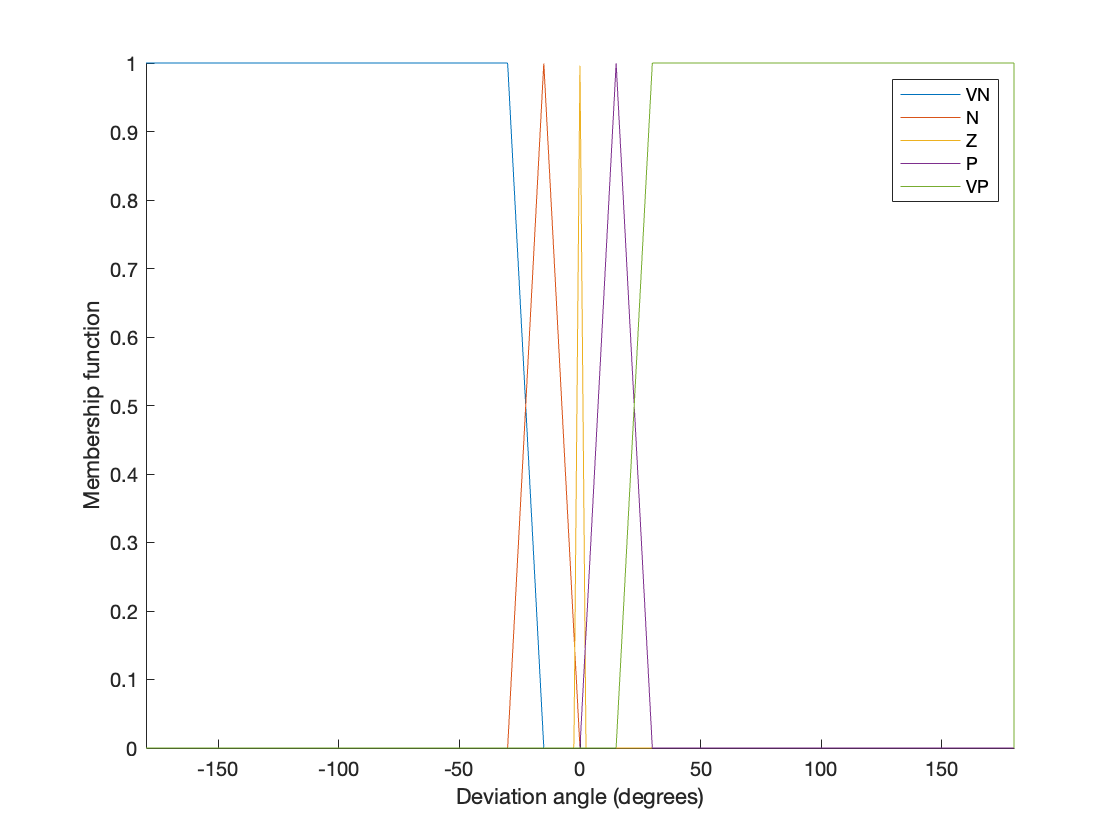
\includegraphics[scale=0.35]{images/fuzzify.png}
    \caption{ Membership functions of the defined sets }
    \label{fig:fuzzify}
\end{figure}

The first step our controller takes, is to determine the extent to which the state of the system belongs to each of the defined sets. We defined the membership functions of the class as shown in fig. \ref{fig:fuzzify}. The width of the zero class alone is smaller, since we want to take action more even for small deviations from the equilibrium point. \\

\begin{figure}[h!]
    \centering
    \includegraphics[scale=0.35]{images/Action.png}
    \caption{ Control action vs System state }
    \label{fig:Action}
\end{figure}

We want to define what action our controller should take for each set. Hence we defined control rules for our controller. We then weight this control rule's action by how much the systems state belongs to the set we are considering. We now sum all the actions we need to take, basically for all the sets we have defined. Effectively, the controller responds to the state of the system as shown in fig. \ref{fig:Action}. \\

The defined rules are summarized below:
\begin{center}
\begin{tabular}{ | c | c | c |}
	\hline
	Fuzzy set & Range		&  Control Action \\
	\hline 
	\hline
	VN 		& -180 to -15	&  4 \\
	\hline
	N		& -30  to 0	&  2 \\  
	\hline
	Z		& -5 to 5		&  0 \\
	\hline
	P		&  0 to  30	& -2 \\
	\hline
	VP		& 15 to 180	& -4 \\
	\hline
\end{tabular}
\end{center}

Lastly, we want to translate this notion of an output that we have into a real-world action. We need to defuzzify our inference. This was done by using a constant $K_{defuz}$, which was set to be 0.09 by trial and error. \\

For the design of this controller, the referenced online course was consulted heavily, since we were unfamiliar with concepts of fuzzy logic \cite{ref1}. 



